\documentclass{llncs}

\pagestyle{plain}

\usepackage[left=3.5cm,right=3.5cm,top=3.5cm,bottom=3cm]{geometry}

\usepackage[english]{babel}
\usepackage[dvipsnames]{xcolor}
\usepackage{graphicx}
\usepackage{listings}
\usepackage{times}
\usepackage{xspace}
\usepackage{booktabs}
\usepackage{subfigure}
\usepackage{hyperref}
\usepackage{wrapfig}
\usepackage{psharp}

\urlstyle{rm}

%\newcommand{\TODO}[1]{\textcolor{red}{\textbf{TODO:} #1}}
%\newcommand{\PDComment}[1]{\textcolor{cyan}{\textbf{PD:} #1}}

% General macros
\newcommand{\ps}{P\#\xspace}
\newcommand{\cs}{C\#\xspace}

\newcommand{\newparagraph}[1]{\smallskip\noindent\textbf{#1 }}

\begin{document}

\title{Getting Started with the \ps Framework}

\author{Pantazis Deligiannis$^1$, Akash Lal$^2$, Shaz Qadeer$^3$}
\institute{$^1$ \textsf{p.deligiannis@imperial.ac.uk}, \emph{Imperial College London}, UK\\$^2$ \textsf{akashl@microsoft.com}, \emph{Microsoft Research}, India\\$^3$ \textsf{qadeer@microsoft.com}, \emph{Microsoft Research}, USA}

\maketitle

\section{Introduction}
\label{sec:intro}

\ps~\cite{deligiannis2015psharp}\cite{deligiannis2016psharp} is an advanced systematic testing framework, designed to significantly ease the process of developing and testing asynchronous reactive applications (i.e.\ distributed systems and web services) in Microsoft's .NET platform. \ps works as follows:

\begin{itemize}
\item Provides an API for writing \emph{test harnesses}, specifying \emph{safety} and \emph{liveness properties}, and \emph{modeling} the individual components of a large system as \emph{communicating state-machines} (which is a similar concept to actors).

\item During testing, the \ps runtime takes control of the \ps test harness (which drives the system-under-test) and all the modeled components, and systematically explores all interleavings between asynchronous events, as well as other declared sources of nondeterminism (e.g.\ timeouts and failures), to find bugs, such as local and global safety and liveness property violations, and runtime exceptions.

\item \ps can be optionally used for development of applications that will get deployed in production. \ps provides a runtime where the execution of the \ps state-machines is not controlled. This runtime is a thin layer built on top of TPL.
\end{itemize}

\newparagraph{Programming model} \ps is built on top of the Roslyn\footnote{\textcolor{blue}{\url{https://github.com/dotnet/roslyn}}} compiler and provides new \cs language primitives (which are largely based on Microsoft's P~\cite{desai2013p} programming language) for creating machines, sending events from one machine to another, and writing assertions about system properties. Each machine has an input queue, states, state transitions, event handlers, fields and methods. Machines run concurrently with each other, each executing an event handling loop that dequeues an event from the input queue and handles it by executing a sequence of operations. Each operation might update a field, create a new machine, or send an event to another machine. In \ps, create machine operations and send operations are non-blocking. In the case of a send operation the message is simply enqueued into the input queue of the target machine.\\

\newparagraph{Usage} There are many different ways that someone can use \ps to test existing systems, or build new highly-reliable ones:

\begin{itemize}
\item \ps can be used just for systematically testing an existing message-passing system, by modeling its environment (e.g.\ a client) and/or components of the system.

\item The \emph{surface syntax} of \ps can be used to write an entire system from scratch. The surface \ps syntax directly extends \cs with new language constructs, which allows for rapid prototyping. However, to use the surface syntax, a developer has to use the \ps compiler, which is built on top of Roslyn. The main disadvantage of this approach is that \ps does not yet fully integrate with the Visual Studio integrated development environment (IDE), and thus does not support high-productivity features such as IntelliSense (e.g. for auto-completition and automated refactoring).

\item \ps can be used as a \cs library to write an entire system from scratch. This approach is slightly more verbose than the above, but allows full integration with Visual Studio. Note that most examples in this guide will use the \ps surface syntax, since it is less verbose. See \S\ref{sec:basics:example} for an example of using \ps as a \cs library.
\end{itemize}

\newparagraph{Repository} The \ps framework is publicly available as open-source and can be found at its git repository at \textcolor{blue}{\url{https://github.com/p-org/PSharp}}.\\

\noindent
In the rest of this guide, we first introduce the basic features of a \ps program (see \S\ref{sec:basics}) and then discuss how \ps can be embedded in \cs code (see \S\ref{sec:interop}). Next, we present an example of a simple program using both the \ps surface syntax and \ps as a library (see \S\ref{sec:basics:example}). We then present the more advanced features of \ps (see \S\ref{sec:advanced}). Next, we illustrate how someone can write safety properties in \ps (see \S\ref{sec:safetyproperties}), which can be systematically checked for bugs. Finally, we provide an overview of the tools for compiling and systematically testing a \ps program.

% Basic features of a P# program
\section{Basic features of a \ps program}
\label{sec:basics}

A \ps program is a collection of \texttt{event} and \texttt{machine} declarations and, optionally, other top-level \cs declarations, such as \texttt{class} and \texttt{struct}. All top-level declarations must be declared inside a \texttt{namespace}, as in \cs. If someone uses the \ps high-level syntax, then events and machines must be declared inside a \texttt{.psharp} file, while \cs top-level declarations must be declared in a \texttt{.cs} file. On the other hand, if someone uses \ps as a \cs library, all the code must be written inside a \texttt{.cs} file.

State machines are first-class citizens of the \ps language and can be declared in the following way:

\begin{psharpNoLines}
machine Server { ... }
\end{psharpNoLines}

\noindent
The above code snippet declares a \ps machine named \texttt{Server}. Machine declarations are similar to class declarations in \cs, and thus can contain an arbitrary number of fields and methods. For example, the below code snippet declares the field \texttt{client} of type \texttt{machine}. An object of this type contains a reference to a machine instance.

\begin{psharpNoLines}
machine Server {
  machine client;
}
\end{psharpNoLines}

\noindent
The main difference between a class and a machine declaration is that the latter must also declare one or more \emph{states}:

\begin{psharpNoLines}
machine Server {
  machine client;
  start state Init { ... }
  state Active { ... }
}
\end{psharpNoLines}

\noindent
The above declares two states in the \texttt{Server} machine: \texttt{Init} and \texttt{Active}. The \ps developer must use the \texttt{start} modifier to declare an \emph{initial} state, which will be the first state that the machine will transition to upon instantiation. In this example, the \texttt{Init} state has been declared as the initial state of \texttt{Server}. Note that only a single state is allowed to be declared as an initial per machine. A \texttt{state} declaration can optionally contain a number of state-specific actions, as seen in the following code snippet:

\begin{psharpNoLines}
state SomeState {
  entry { ... }
  exit { ... }
}
\end{psharpNoLines}

\noindent
A code block indicated by \texttt{entry} \{ ...\ \} denotes an action that will be executed when the machine transitions to the state, while a code block indicated by \texttt{exit} \{ ...\ \} denotes an action that will be executed when the machine leaves the state. Actions in \ps are essentially \cs methods with no input parameters and \texttt{void} return type. \ps actions can contain arbitrary \ps and \cs statements. However, since we want to explicitly declare all sources of asynchrony using \ps, we only allow the use of \emph{sequential} \cs code inside a \ps machine.\footnote{In practise, we just assume that the \cs code is sequential, as it would be very challenging to impose this rule in real life programs (e.g.\ a developer could use an external library).} An example of an \texttt{entry} action is the following:

\begin{psharpNoLines}
entry {
  this.client = create(Client);
  send(this.client, Config, this);
  send(this.client, Ping);
  raise(Unit);
}
\end{psharpNoLines}

\noindent
The above action contains the three most important \ps statements. The \texttt{create} statement is used to create a new instance of the \texttt{Client} machine. A reference to this instance is stored in the \texttt{client} field. Next, the \texttt{send} statement is used to send an event (in this case the events \texttt{Config} and \texttt{Ping}) to a target machine (in this case the machine whose address is stored in the field \texttt{client}).

When an event is being send, it is enqueued in the event queue of the target machine, which can then dequeue the received event, and handle it asynchronously from the sender machine. Finally, the \texttt{raise} statement is used to send an event to the caller machine (i.e. to itself). When a machine raises an event, the raised event is not enqueued as in the case of \texttt{send}; instead, the machine terminates execution of the enclosing code block and handles the event immediately. In \ps, events (e.g.\ \texttt{Ping}, \texttt{Unit} and \texttt{Config} in the above example) can be declared as follows:

\begin{psharpNoLines}
event Ping;
event Unit;
event Config (target: machine);
\end{psharpNoLines}

\noindent
A \ps machine can send data (scalar values or references) to a target machine, as the payload of an event. Such an event must specify the type of the payload in its declaration (as in the case of the \texttt{Config} event above). A machine can also send data to itself (e.g.\ for processing in a later state) using \texttt{raise}.

In the previous example, the \texttt{Server} machine sends \texttt{this} (i.e.\ a reference to the current machine instance) to the \texttt{client} machine. The receiver (in our case \texttt{client}) can retrieve the sent data by using the keyword \texttt{trigger} (or \texttt{ReceivedEvent} when using \ps as a \cs library), which is a handle to the received event, casting \texttt{trigger} to the expected event type (in this case \texttt{Config}), and then accessing the payload as a field of the received event.

As discussed earlier, the \texttt{create} and \texttt{send} statements are non-blocking. The \ps runtime will take care of all the underlying asynchrony using the Task Parallel Library and, thus, the developer does not need to explicitly create and manage tasks.

Besides the \texttt{entry} and \texttt{exit} declarations, all other declarations inside a \ps state are related to \emph{event-handling}, which is a key feature of \ps. An event-handler declares how a \ps machine should \emph{react} to a received event. One such possible reaction is to create one or more machine instances, send one or more events, or process some local data. The two most important event-handling declarations in \ps are the following:

\begin{psharpNoLines}
state SomeState {
  on Unit goto AnotherState;
  on Pong do SomeAction;
}
\end{psharpNoLines}

\noindent
The declaration \texttt{on Unit goto AnotherState} indicates that when the machine receives the \texttt{Unit} event in \texttt{SomeState}, it must handle the event by exiting the state and transitioning to \texttt{AnotherState}. The declaration \texttt{on Pong do SomeAction} indicates that the \texttt{Pong} event must be handled by invoking the action \texttt{SomeAction}. Each event can be associated with at most one handler in a particular state of a machine. \ps also supports \emph{anonymous} event-handlers. For example, the declaration \texttt{on Pong do} \{ ...\ \} is an anonymous event-handler, which states that the block of statements between the braces must be executed when event \texttt{Pong} is dequeued.

\ps also supports specifying invariants (i.e.\ assertions) on the local state of a machine. The developer can achieve this by using the \texttt{assert} statement, which accepts as input a predicate that must always hold in that specific program point, e.g.\ \texttt{assert(k == 0)}, which holds if the integer \texttt{k} equals to 0.

% A Simple Example Program
\subsection{A Simple Example Program}
\label{sec:basics:example}

The following \ps program shows a \texttt{Client} machine and a \texttt{Server} machine that communicate asynchronously by exchanging \texttt{Ping} and \texttt{Pong} events:

\begin{psharp}
namespace PingPong {
  event Ping; // Client sends this event to the Server
  event Pong; // Server sends this event to the Client
  event Unit; // Event used for local transitions
  
  // Event used for configuration, can take a payload
  event Config (target: machine);
  
  machine Server {
    machine client;
  
    start state Init {
      entry {
        // Instantiates the Client
        this.client = create(Client);
        // Sends event to client to configure it
        send(this.client, Config, this);
        raise(Unit); // Sends an event to itself
      }
      
      on Unit goto Active; // Performs a state transition
    }
  
    state Active {
      on Ping do {
        // Sends a Pong event to the Client
        send(this.client, Pong);
      };
    }
  }
  
  machine Client {
    machine server;
  
    start state Init {
      on Config do Configure; // Handles the event
      on Unit goto Active; // Performs a state transition
    }
    
    void Configure() {
      // Receives reference to Server
      this.server = (trigger as Config).target;
      raise(Unit); // Sends an event to itself
    }
  
    state Active {
      entry {
        SendPing();
      }
      on Pong do SendPing;
    }
  
    void SendPing() {
      // Sends a Ping event to the Server
      send(this.server, Ping);
    }
  }
  
  public class HostProgram {
    static void Main(string[] args) {
      PSharpRuntime.Create().CreateMachine(typeof(Server));
      Console.ReadLine();
    }
  }
}
\end{psharp}

\noindent
In the above example, the program starts by creating an instance of the \texttt{Server} machine (line 61). The implicit constructor of each \ps machine initializes the internal to the \ps runtime data of the machine, including the event queue, a set of available states, and a map from events to event-handlers per state.

After the \texttt{Server} machine has initialized, the \ps runtime executes the \texttt{entry} action of the initial (\texttt{Init}) state of \texttt{Server}, which first creates an instance of the \texttt{Client} machine (line 15), then sends the event \texttt{Config} to the \texttt{Client} machine (line 17), with the \texttt{this} reference as a payload, and then raises the event \texttt{Unit} (line 18). As mentioned earlier, when a machine calls \texttt{raise}, it exits the currently executing action, and immediately handles the raised event (bypassing the queue). In this case, the \texttt{Server} machine handles \texttt{Unit} by transitioning to the \texttt{Active} state (line 21).

\texttt{Client} starts executing (asynchronously) when it is created by \texttt{Server}. The \texttt{Client} machine stores the received payload (which is a reference to the \texttt{Server} machine) in the \texttt{server} field (line 42), and then raises \texttt{Unit} to transition to the \texttt{Active} state. In the new state, \texttt{Client} calls the \texttt{SendPing} method to send a \texttt{Ping} event to \texttt{Server} (line 55). In turn, the \texttt{Server} machine dequeues \texttt{Ping} and handles it by sending a \texttt{Pong} event to \texttt{Client} (line 27), which subsequently responds by sending a new \texttt{Ping} event to \texttt{Server}. This asynchronous exchange of \texttt{Ping} and \texttt{Pong} events continues indefinitely.

% Interoperability
\section{Interoperability Between \ps and \cs}
\label{sec:interop}

Because \ps is built on top of the \cs language, the entry point of a \ps program (i.e.\ the first machine that the \ps runtime will instantiate and execute) must be explicitly declared inside a host \cs program (typically in the \texttt{Main} method), as follows:

\begin{psharpNoLines}
using Microsoft.PSharp;
public class HostProgram {
  static void Main(string[] args) {
    PSharpRuntime.Create().CreateMachine(typeof(Server));
    Console.ReadLine();
  }
}
\end{psharpNoLines}

\noindent
The developer must first import the \ps runtime library (\texttt{Microsoft.PSharp.dll}), then create a \texttt{PSharpRuntime} instance, and finally invoke the \texttt{CreateMachine} runtime method to instantiate the first \ps machine (\texttt{Server} in the above example).

The \texttt{CreateMachine} method is part of the .NET interoperability API (a set of methods for calling \ps from native \cs code) that is exposed by \texttt{PSharpRuntime}. This method accepts as a parameter the type of the machine to be instantiated, and returns an object of the \texttt{MachineId} type, which contains a reference to the created \ps machine. Because \texttt{CreateMachine} is an asynchronous method, we call the \texttt{Console.ReadLine} method, which pauses the main thread until a console input has been given, so that the host \cs program does not exit prematurely.

The \texttt{PSharpRuntime} .NET interoperability API also provides the \texttt{SendEvent} method for sending events to a \ps machine from native \cs. This method accepts as parameters an object of type \texttt{MachineId}, an event and an optional payload. Although the developer has to use \texttt{CreateMachine} and \texttt{SendEvent} to call \ps code from native \cs, the opposite is straightforward, as it only requires accessing a \cs object from \ps code.

The example of \S\ref{sec:basics:example} can be written using \ps as a \cs library as follows:

\begin{psharp}
// PingPong.cs
using System;
using Microsoft.PSharp;

namespace PingPong {
  class Unit : Event { }
  class Ping : Event { }
  class Pong : Event { }
  
  class Config : Event {
    public MachineId Target;
    public Config(MachineId target) : base() {
      this.Target = target;
    }
  }
  
  class Server : Machine {
    MachineId Client;
    
    [Start]
    [OnEntry(nameof(InitOnEntry))]
    [OnEventGotoState(typeof(Unit), typeof(Active))]
    class Init : MachineState { }
    
    void InitOnEntry() {
      this.Client = this.CreateMachine(typeof(Client));
      this.Send(this.Client, new Config(this));
      this.Raise(new Unit());
    }
    
    [OnEventDoAction(typeof(Pong), nameof(SendPing))]
    class Active : MachineState {
      protected override void OnEntry() {
        (this.Machine as Server).SendPing();
      }
    }
    
    void SendPing() {
      this.Send(this.Client, new Ping());
    }
  }
  
  class Client : Machine {
    MachineId Server;
    
    [Start]
    [OnEventGotoState(typeof(Unit), typeof(Active))]
    [OnEventDoAction(typeof(Config), nameof(Configure))]
    class Init : MachineState { }
    
    void Configure() {
      this.Server = (this.ReceivedEvent as Config).Trigger;
      this.Raise(new Unit());
    }
    
    [OnEventDoAction(typeof(Ping), nameof(SendPong))]
    class Active : MachineState { }
    
    void SendPong() {
      this.Send(this.Server, new Pong());
    }
  }
  
  public class Program {
    static void Main(string[] args) {
      PSharpRuntime.CreateMachine(typeof(Server));
      Console.ReadLine();
    }
  }
}
\end{psharp}

The programmer can use \ps as a library by importing the \texttt{Microsoft.PSharp.dll} library. A \ps machine can be declared by creating a \cs \texttt{class} that inherits from the type \texttt{Machine} (provided by the \ps library). A state can be declared by creating a \texttt{class} that inherits from the type \texttt{MachineState}. This state class must be nested inside a machine class (no other class besides a state can be nested inside a machine class). The start state can be declared using the \texttt{[Start]} attribute.

A state transition can be declared using the \texttt{[OnEventGotoState(...)]} attribute, where the first argument of the attribute is the type of the received event and the second argument is the type of the target state. An optional third argument, is a string that denotes the name of the method to be executed after exiting the state and before entering the new state. Likewise, an action handler can be declared using the \texttt{[OnEventDoAction(...)]} attribute, where the first argument of the attribute is the type of the received event and the second argument is the name of the action to be executed. All \ps statements (e.g. \texttt{send} and \texttt{raise}) are exposed as method calls of the \texttt{Machine} and \texttt{MachineState} classes.

Note that even when using \ps as a \cs library, the program has to still be compiled using the \ps compiler as the compiler performs some important static checking to find \ps syntax-related errors and rewriting (e.g.\ a \texttt{return} statement is instrumented after a \texttt{raise}).

% Advanced features of P#
\section{Advanced features of \ps}
\label{sec:advanced}

The following is a discussion of more advanced features of \ps, such as explicit termination of machines, modeling components and the environment of a system, and specifying safety and liveness properties.

\subsection{Explicit termination of \ps machines}
\label{sec:termination}

In order to terminate a \ps machine explicitly, it must dequeue a special event named \texttt{halt}, which is provided by \ps (the user cannot declare it). A \texttt{halt} event (\texttt{Halt} when using \ps as a library) can be raised and/or send to another machine. Termination of a machine due to an unhandled \texttt{halt} event is valid behavior (the \ps runtime does not report an error). From the point of view of formal operational semantics, a halted machine is fully receptive and consumes any event that is sent to it. The \ps runtime implements this semantics efficiently by cleaning up resources allocated to a halted machine and recording that the machine has halted. An event sent to a halted machine is simply dropped. A halted machine cannot be restarted; it remains halted forever.

% Modeling System Components using P#
\subsection{Modeling System Components using \ps}
\label{sec:advanced:modeling}

\begin{figure*}[t]
\centering
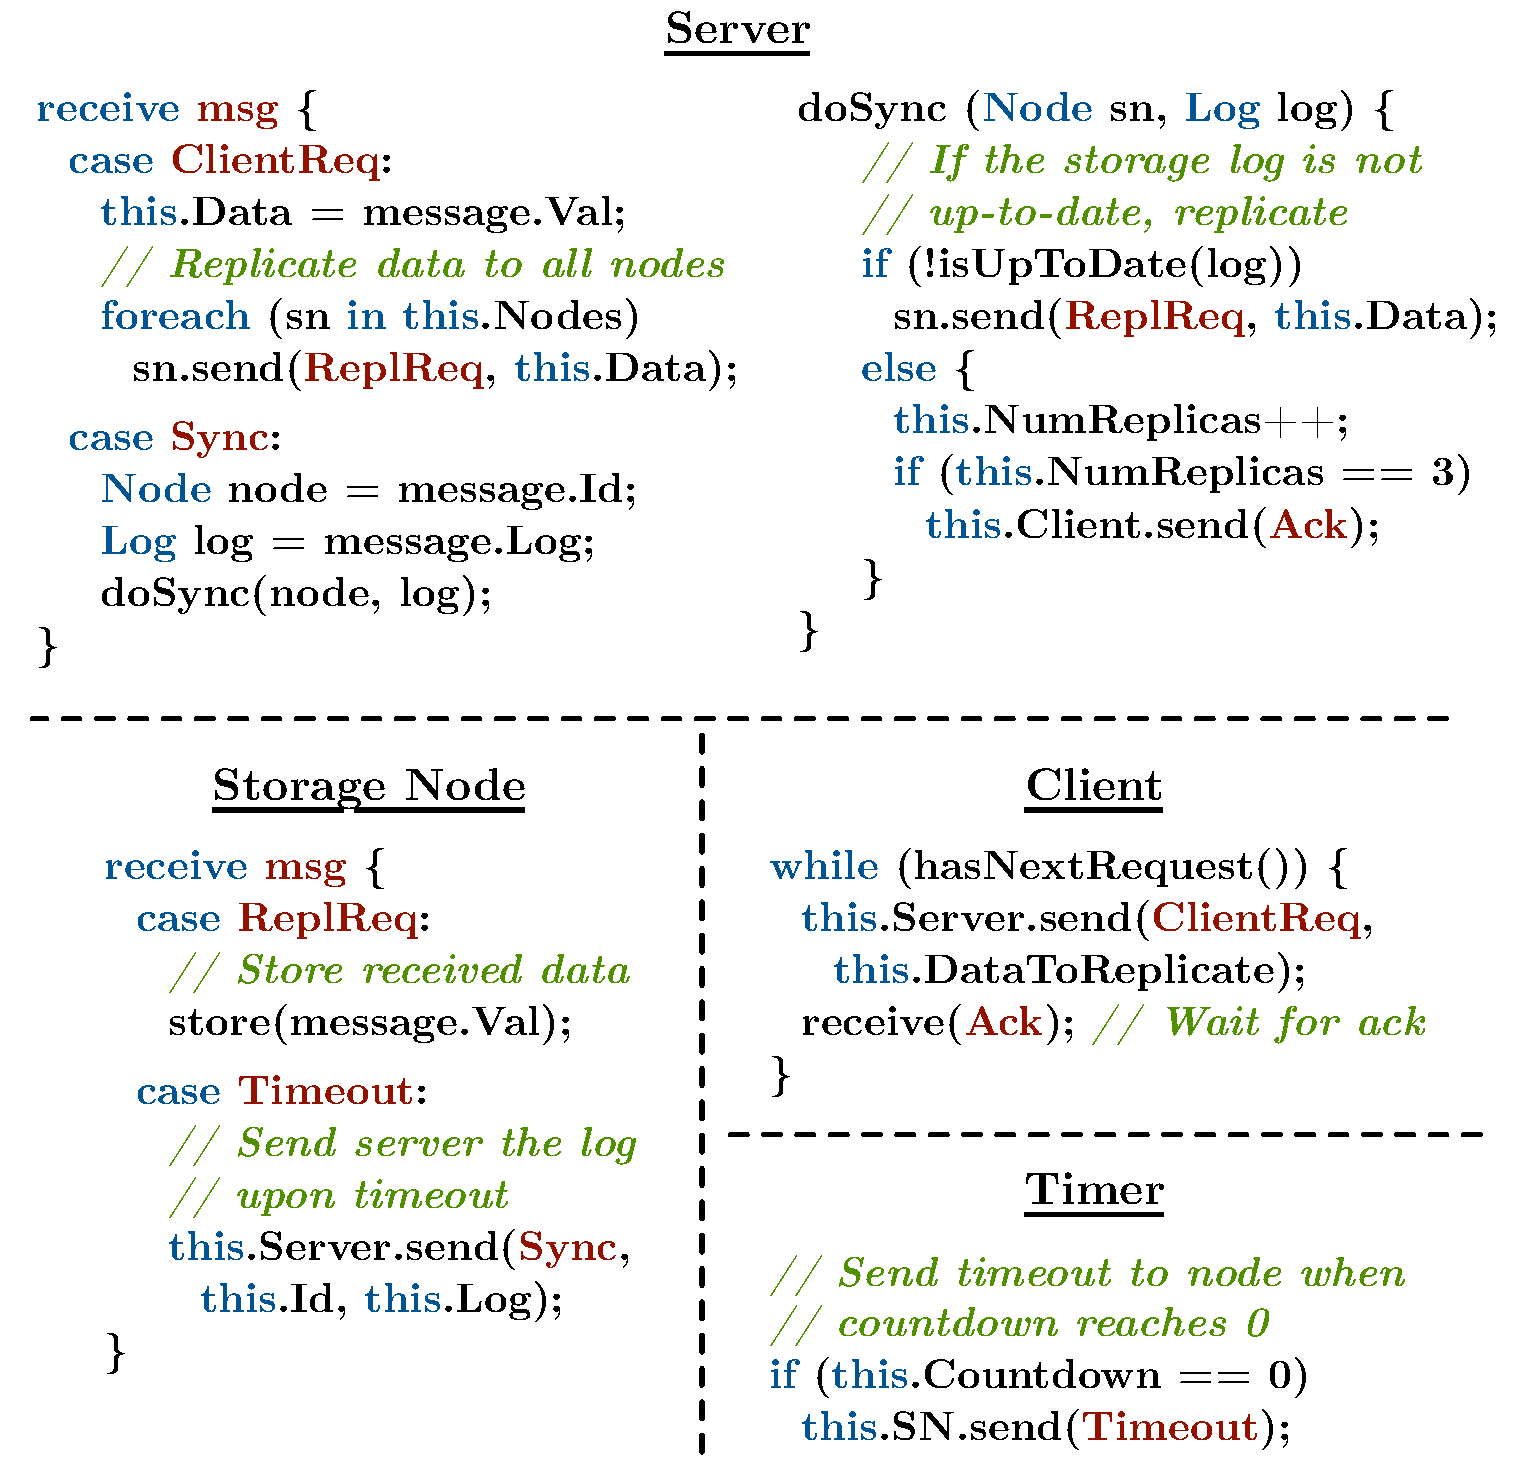
\includegraphics[width=.7\linewidth]{figures/example_code}
\caption[Pseudocode of a simple distributed storage system]{Pseudocode of a simple distributed storage system that is responsible for replicating the data sent by a client.}
\label{fig:example}
\end{figure*}

Figure~\ref{fig:example} presents the pseudocode of a simple distributed storage system that was contrived for the purposes of explaining our \ps testing methodology. The system consists of a client, a server and three storage nodes (SNs). The client sends the server a \texttt{ClientReq} message that contains data to be replicated (\texttt{DataToReplicate}), and then waits to get an acknowledgement (by calling the \texttt{receive} method) before sending the next request. When the server receives \texttt{ClientReq}, it first stores the data locally (in the \texttt{Data} field), and then broadcasts a \texttt{ReplReq} message to all SNs. When an SN receives \texttt{ReplReq}, it handles the message by storing the received data locally (by calling the \texttt{store} method). Each SN has a timer installed, which sends periodic \texttt{Timeout} messages. Upon receiving \texttt{Timeout}, an SN sends a \texttt{Sync} message to the server that contains the storage log. The server handles the \texttt{Sync} message by calling the \texttt{isUpToDate} method to check if the SN log is up-to-date. If it is not, the server sends a repeat \texttt{ReplReq} message to the outdated SN. If the SN log is up-to-date, then the server increments a replica counter by one. Finally, when there are three replicas available, the server sends an \texttt{Ack} message to the client.

There are two bugs in this example. The first bug is that the server does not keep track of unique replicas. The replica counter increments upon each up-to-date \texttt{Sync}, even if the syncing SN is already considered a replica. This means that the server might send an \texttt{Ack} message when fewer than three replicas exist, which is erroneous behaviour. The second bug is that the server does not reset the replica counter to 0 upon sending an \texttt{Ack} message. This means that when the client sends another \texttt{ClientReq} message, it will never receive \texttt{Ack}, and thus block indefinitely. To systematically test this example, the developer must first create a \ps test harness, and then specify the correctness properties of the system. Figure~\ref{fig:example:model} illustrates a test harness that can find the above two bugs.

\begin{figure}[t]
\centering
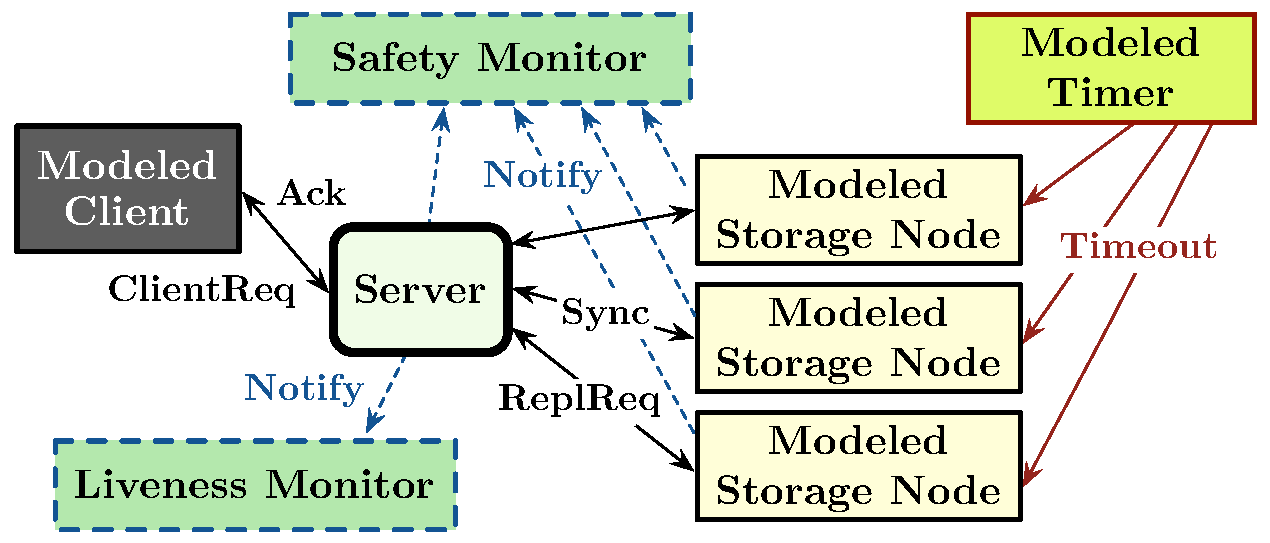
\includegraphics[width=.7\linewidth]{figures/example}
\caption[The \ps test harness for the example in Figure~\ref{fig:example}]{The \ps test harness for the example in Figure~\ref{fig:example}.}
\label{fig:example:model}
\end{figure}

Each box in the figure represents a concurrently running \ps machine, while an arrow represents an event being sent from one machine to another. We use three kinds of boxes: (i) a box with rounded corners and thick border denotes a real component wrapped inside a \ps machine; (ii) a box with thin border denotes a modeled component; and (iii) a box with dashed border denotes a special \ps machine used for safety or liveness checking (see \S\ref{sec:advanced:safety} and \S\ref{sec:advanced:liveness}).

We do not model the server component since we want to test its actual implementation. The server is wrapped inside a \ps machine, which is responsible for (i) sending the system messages (as payload of a \ps event) via the \ps \texttt{send(...)} method, instead of the real network, and (ii) delivering received messages to the wrapped component. We model the SNs so that they store data in memory rather than on disk (which can be inefficient during testing). We also model the client so that it can drive the system by repeatedly sending a nondeterministically generated \texttt{ClientReq}, and then waiting for an \texttt{Ack} event. Finally, we model the timer so that \ps takes control of all time-related nondeterminism in the system. This allows the \ps testing engine to control when a \texttt{Timeout} event will be sent to the SNs during testing, and (systematically) explore different schedules.

\ps uses object-oriented language features such as interfaces and dynamic method dispatch to connect the real code with the modeled code. Developers in industry are used to working with such features, and heavily employ them in testing production systems. In our experience, this significantly lowers the bar for engineering teams inside Microsoft to embrace \ps for testing.

\subsection{Writing safety properties}
\label{sec:advanced:safety}

Safety property specifications generalize the notion of source code assertions; a safety property violation is a finite trace leading to an erroneous state. \ps supports the usual assertions for specifying safety properties that are local to a \ps machine (see \S\ref{sec:basics}), and also provides a way to specify global assertions in the form of a \emph{safety monitor}, a special \ps machine that can receive, but not send, events.

A safety monitor maintains local state that is modified in response to events received from ordinary (non-monitor) machines. This local state is used to maintain a history of the computation that is relevant to the property being specified. An erroneous global behavior is flagged via an assertion on the private state of the safety monitor. Thus, a monitor cleanly separates the instrumentation state required for specification (inside the monitor) from the program state (outside the monitor).

The first bug in the example of \S\ref{sec:advanced:modeling} is a safety bug. To find it, the developer can write a safety monitor (see Figure~\ref{fig:example:model}) that contains a map from unique SN ids to a Boolean value, which denotes if the SN is a replica or not. Each time an SN replicates the latest data, it notifies the monitor to update the map. Each time the server issues an \texttt{Ack}, it also notifies the monitor. If the monitor detects that an \texttt{Ack} was sent without three replicas actually existing, a safety violation is triggered. The following code snippet shows the \ps source code for this safety monitor:

\begin{psharp}
monitor SafetyMonitor {
  // Map from unique SNs ids to a boolean value
  // that denotes if a node is replica or not
  Dictionary<int, bool> replicas;

  start state Checking {
    entry {
      var node_ids = (HashSet<int>)payload;
      this.replicas = new Dictionary<int, bool>();
      foreach (var id in node_ids) {
        this.replicas.Add(id, false);
      }
    }
    
    // Notification that the SN is up-to-date
    on NotifyUpdated do {
      var node_id = (int)payload;
      this.replicas[node_id] = true;
    };
    
    // Notification that the SN is out-of-date
    on NotifyOutdated do {
      var node_id = (int)payload;
      this.replicas[node_id] = false;
    };
    
    // Notification that an Ack was issued
    on NotifyAck do {
      // Assert that 3 replicas exist
      assert(this.replicas.All(n => n.Value));
    };
  }
}
\end{psharp}

\subsection{Writing liveness properties}
\label{sec:advanced:liveness}

Liveness property specifications generalize nontermination; a liveness property violation is an infinite trace that exhibits lack of progress. Typically, a liveness property is specified via a temporal logic formula. We take a different approach and allow the developers to write a \emph{liveness monitor}. Similar to a safety monitor, a liveness monitor can receive, but not send, events.

A liveness monitor contains two special states: the \emph{hot} and the \emph{cold} state. The hot state denotes a point in the execution where progress is required, but has not happened yet; e.g.\ a node has failed, but a new one has not launched yet. A liveness monitor transitions to the hot state when it is notified that the system must make progress. A liveness monitor leaves the hot state and enters the cold state when it is notified that the system has progressed. An infinite execution is erroneous if the liveness monitor stays in the hot state for an infinitely long period of time. Our liveness monitors can encode arbitrary temporal logic properties.

A liveness property violation is witnessed by an \emph{infinite} execution in which all concurrently executing \ps machines are \emph{fairly} scheduled. Since it is impossible to generate an infinite execution by executing a program for a finite amount of time, our implementation of liveness checking in \ps approximates an infinite execution using several heuristics. In this work, we consider an execution longer than a large user-supplied bound as an ``infinite'' execution. Note that checking for fairness is not relevant when using this heuristic, due to our pragmatic use of a large bound.

The second bug in the example of \S\ref{sec:advanced:modeling} is a liveness bug. To detect it, the developer can write a liveness monitor (see Figure~\ref{fig:example:model}) that transitions from a hot state, which denotes that the client sent a \texttt{ClientReq} and waits for an \texttt{Ack}, to a cold state, which denotes that the server has sent an \texttt{Ack} in response to the last \texttt{ClientReq}. Each time a server receives a \texttt{ClientReq}, it notifies the monitor to transition to the hot state. Each time the server issues an \texttt{Ack}, it notifies the monitor to transition to the cold state. If the monitor is in a hot state when the bounded infinite execution terminates, a liveness violation is triggered. The following code snippet shows the \ps source code for this liveness monitor:

\begin{psharp}
monitor LivenessMonitor {
  start hot state Progressing {
    // Notification that the server issued an Ack
    on NotifyAck do {
      raise(Unit);
    };
    on Unit goto Progressed;
  }
  
  cold state Progressed {
    // Notification that server received ClientReq
    on NotifyClientRequest do {
      raise(Unit);
    };
    on Unit goto Progressing;
  }
}
\end{psharp}

% The P# compiler
\section{Compiling and Testing \ps Programs}
\label{sec:compilation}

To compile a \ps program, the developer must use the \ps compiler (\texttt{PSharpCompiler.exe}), which is built on top of the Microsoft Roslyn compiler. The \ps compilation process consists of two phases: \emph{parsing} and \emph{rewriting}. In the parsing phase, the input \ps program is parsed using a recursive-descent parser to produce an abstract syntax tree (AST). In the rewriting phase, the \ps compiler traverses the produced AST, and rewrites all \ps statements to native (intermediate) \cs code. Finally, the \ps compiler invokes the Roslyn compiler to build the intermediate \cs program, link it with the \ps runtime library, and produce a .NET executable.

\begin{figure}[t]
\centering
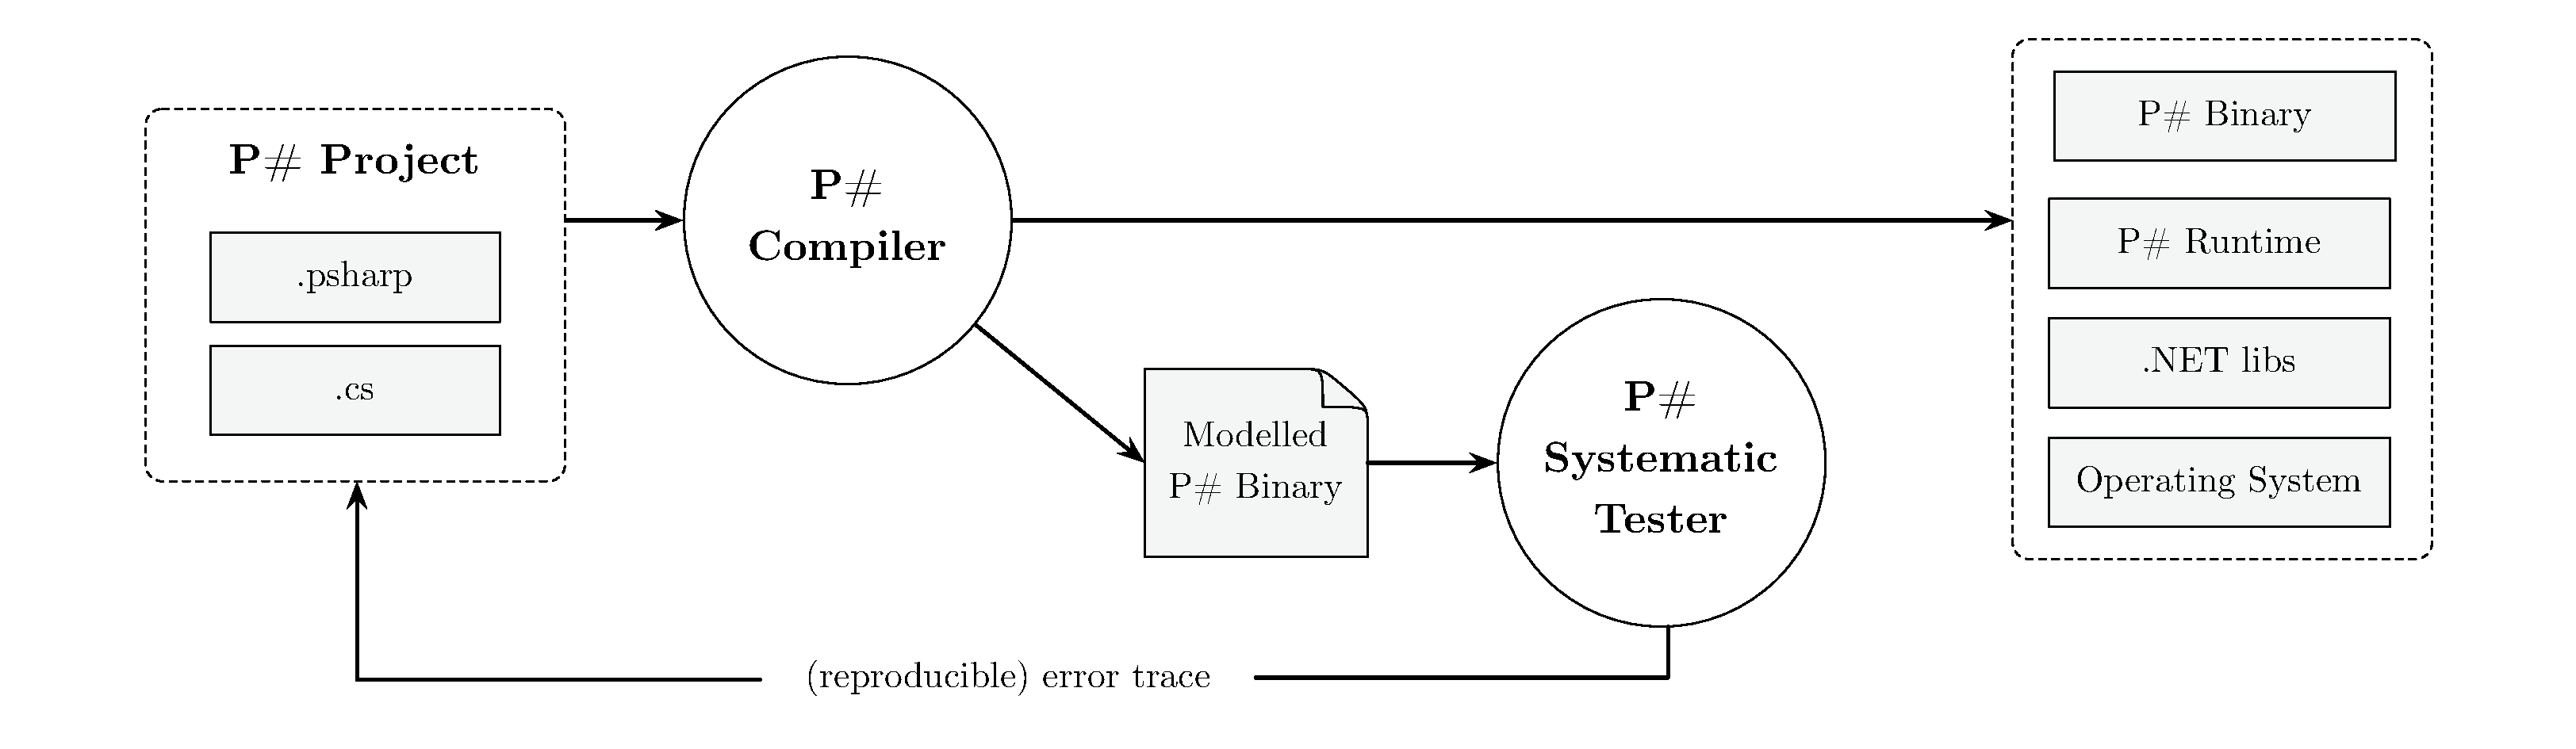
\includegraphics[width=0.95\linewidth]{figures/workflow.pdf}
\caption{The typical \ps workflow.}
\label{fig:workflow}
\end{figure}

To test a \ps program, the developer must use the \texttt{PSharpTester.exe} systematic testing tool (see \textcolor{blue}{\url{https://github.com/p-org/PSharp}} for instructions), or use the \ps systematic testing APIs, as follows:

\begin{psharp}
using System;
using System.Collections.Generic;

using Microsoft.PSharp;
using Microsoft.PSharp.SystematicTesting;
using Microsoft.PSharp.Utilities;

namespace Example
{
    public class Test
    {
        static void Main(string[] args)
        {
            var configuration = Configuration.Create().
                WithLivenessCheckingEnabled().
                WithNumberOfIterations(10).
                WithVerbosityEnabled(2);
            TestingEngine.Create(configuration, Execute).Run();
        }

        [Microsoft.PSharp.Test]
        public static void Execute(PSharpRuntime runtime)
        {
            runtime.CreateMachine(typeof(SomeMachine));
        }
    }
}
\end{psharp}

The developer must first create a \texttt{Configuration} object, which declares testing options such as the number of testing iterations. Next, the developer must create a \texttt{TestingEngine}, passing the configuration instance and the entry point to the test (in our case \texttt{Execute}), which must be annotated with the \texttt{[Microsoft.PSharp.Test]} attribute, as arguments. Finally, the \texttt{Run} method must be invoked to start testing the \ps program.

%\newpage

\bibliographystyle{plain}
\bibliography{references}

\end{document}
